\begin{figure}
%  \begin{subfigure}[b]{.53\textwidth}
%    \centering
%    \begin{tikzpicture}
%
%      \node[inner sep=0pt] (img) at (0,0)
%           {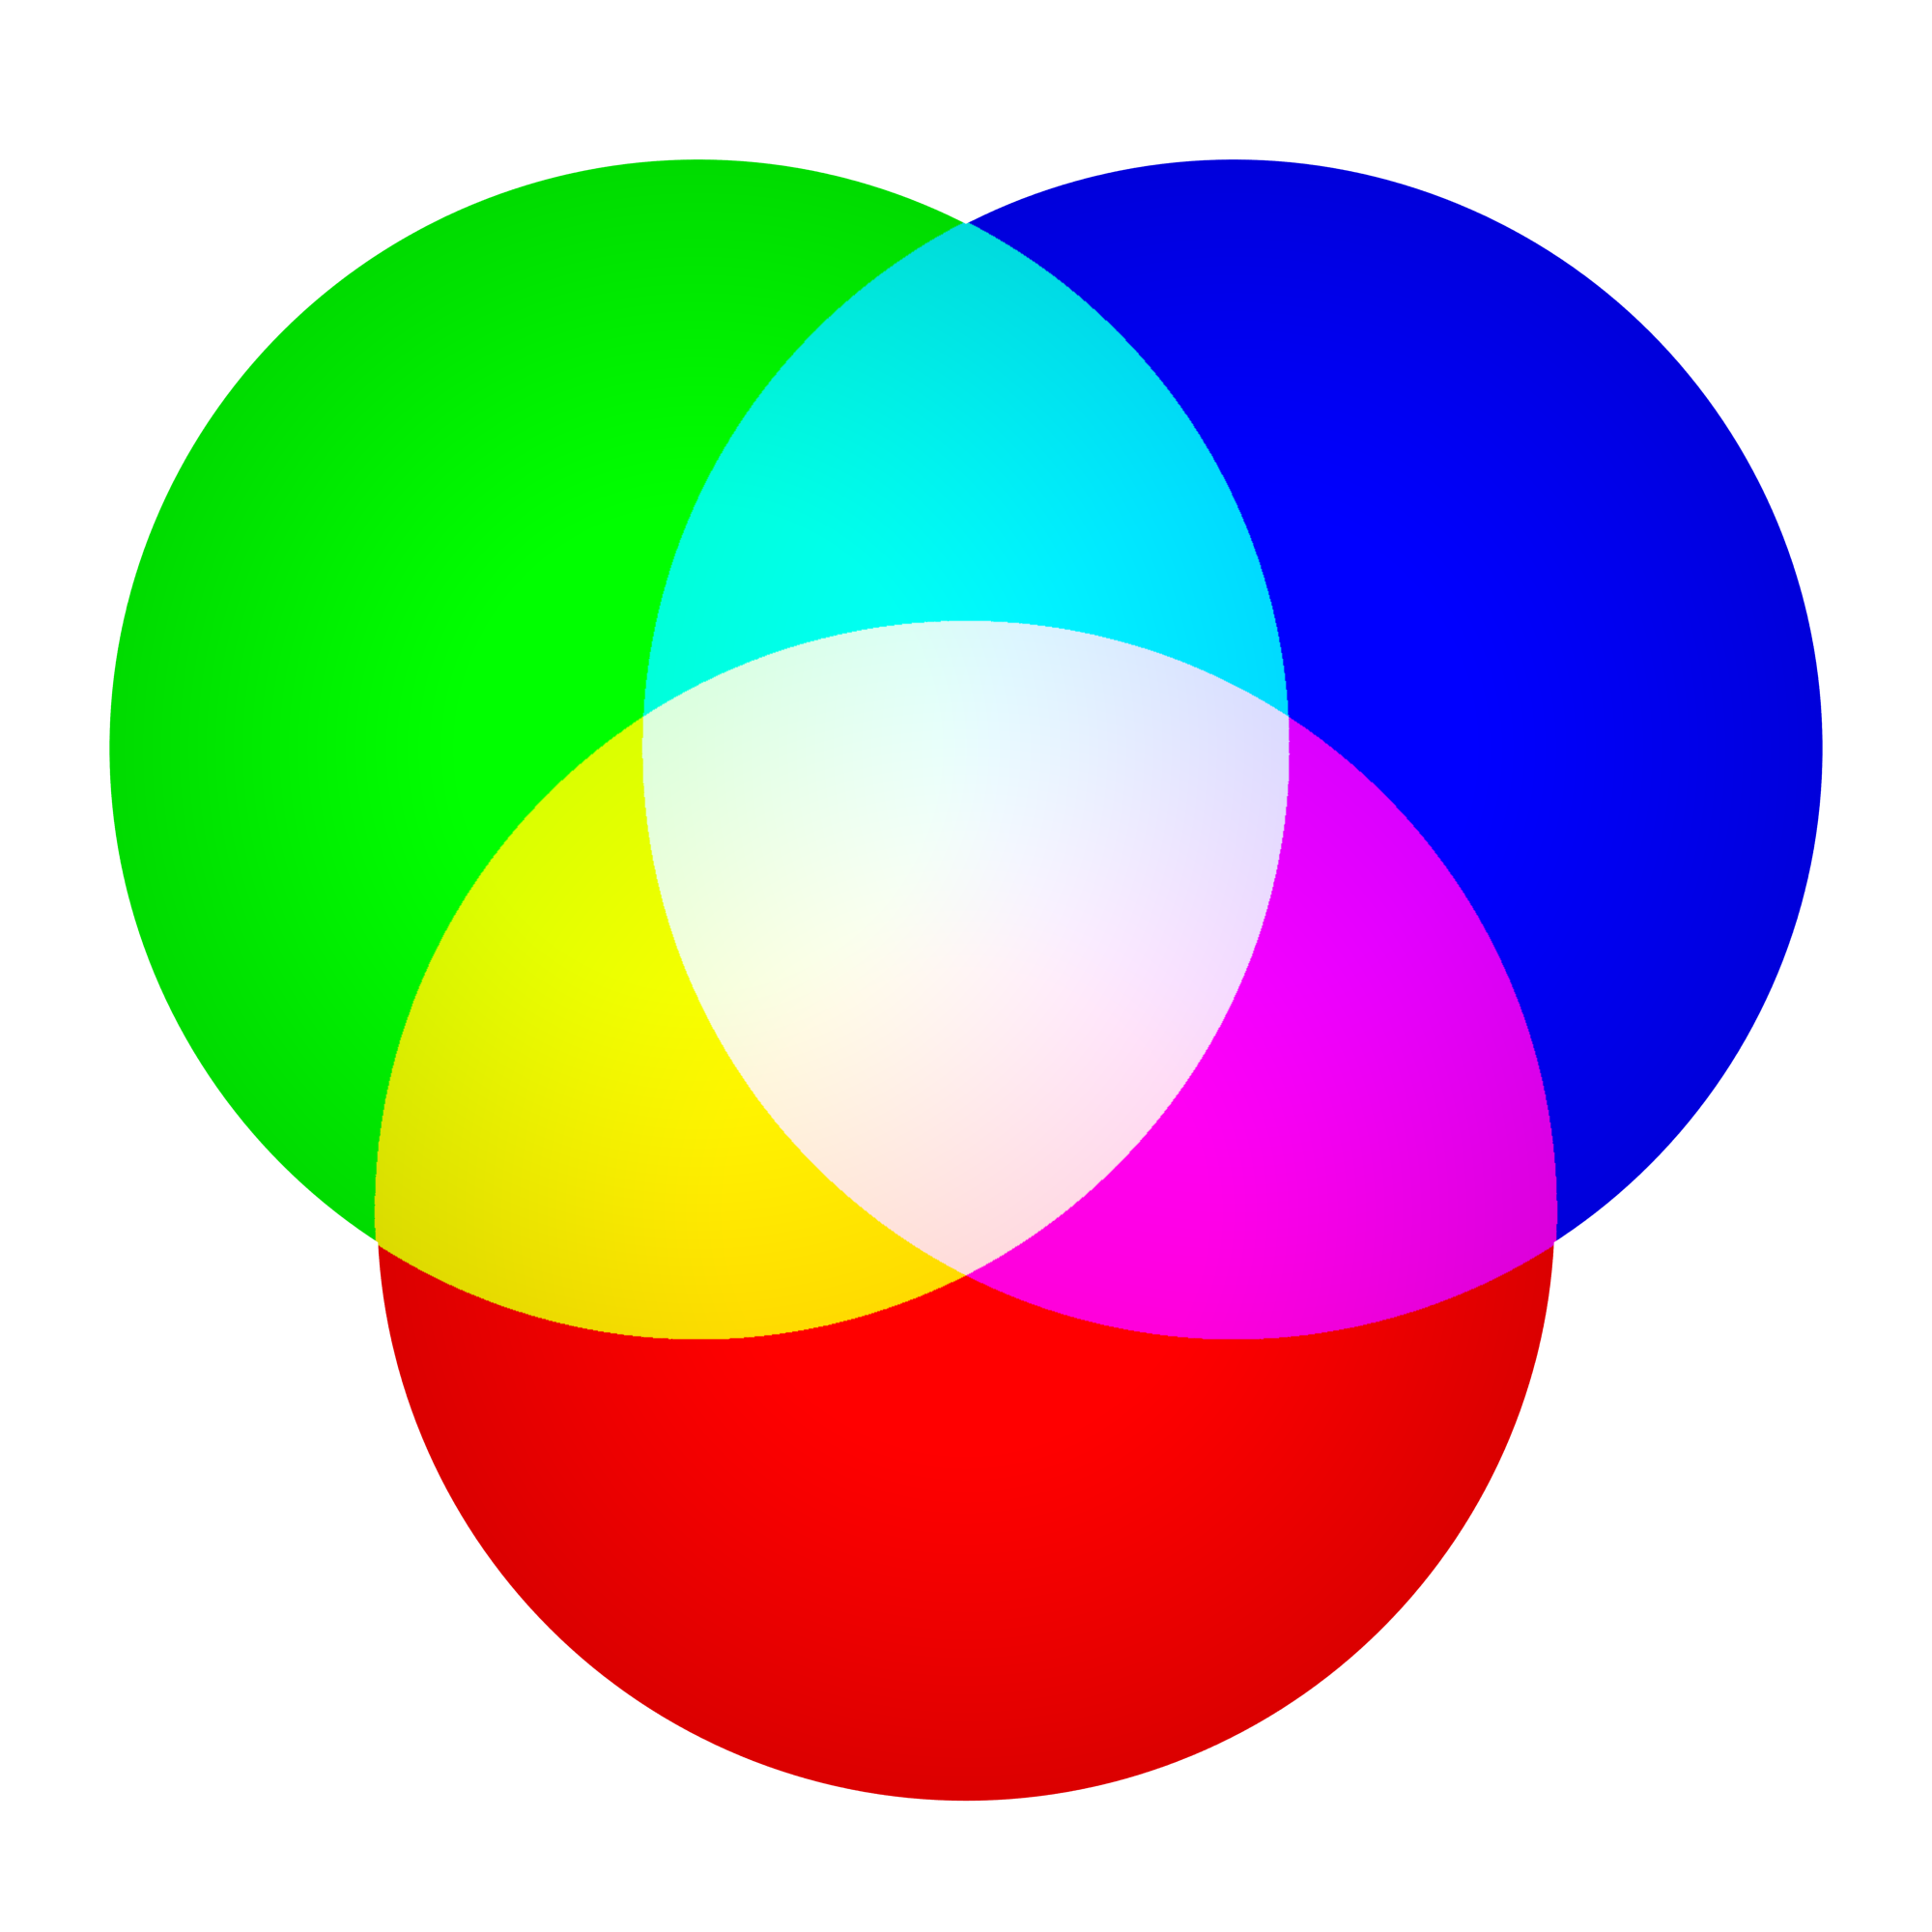
\includegraphics[width=\textwidth]{./img/raw/fw-kleur/colour-wheel1.png}};
%
%      \node (l1) at (0, 0) {Wit};
%      \node (l2) at (0, 1.8) {Cyaan};
%      \node (l3) at (-1.8, 1.3) {Groen};
%      \node (l4) at (1.8, 1.3) {Blauw};
%      \node (l5) at (-1.5, -0.5) {Geel};
%      \node (l6) at (1.5, -0.5) {Magenta};
%      \node (l7) at (0, -2) {Rood};
%    \end{tikzpicture}
%    \label{fig:fw-kleur:illustration}
%    \caption{Mengen van primaire kleuren.}
%  \end{subfigure} %
%  \begin{subfigure}[b]{.46\textwidth}
    \centering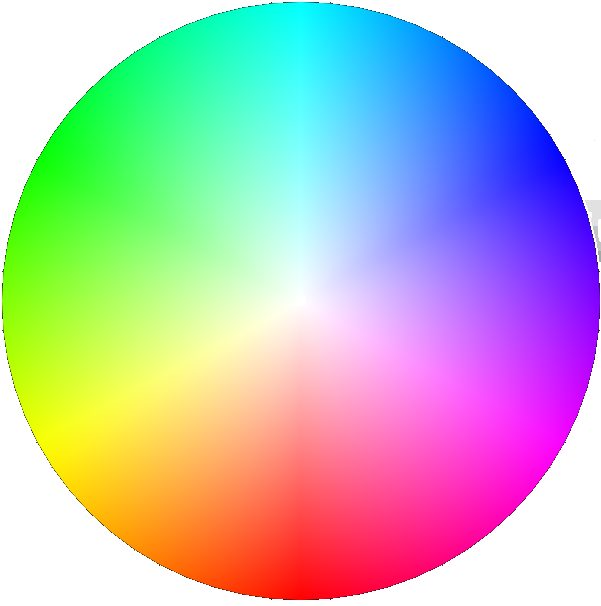
\includegraphics[width=0.4\textwidth]{./img/raw/fw-kleur/colour-wheel2.png}
%    \label{fig:fw-kleur:hsv}
%    \caption{Mengen van alle kleuren.}
%  \end{subfigure} %
  \caption{Het mengen van kleuren volgens een additief model.}
  \label{fig:fw-kleur}
\end{figure}
